%% Final report of the text mining project, Springer Nature template (sn-jnl).
%% Compile on Overleaf with the Springer Nature LaTeX template: see README.md.
\documentclass[pdflatex,sn-mathphys-num]{sn-jnl}

\usepackage{graphicx}
\usepackage{multirow}
\usepackage{amsmath,amssymb}
\usepackage{booktabs}
\usepackage{xcolor}
\usepackage{url}
\usepackage{tikz}
\usetikzlibrary{positioning,arrows.meta,shapes.geometric,calc}
\tikzset{
  reused/.style={draw=black!45, fill=black!7, rounded corners=2pt, align=center, inner sep=3pt, minimum height=8mm},
  added/.style={draw=teal!75!black, fill=teal!14, rounded corners=2pt, align=center, inner sep=3pt, minimum height=8mm, thick},
  flow/.style={-{Stealth[length=2mm]}, thick, black!65},
  cache/.style={cylinder, shape border rotate=90, aspect=0.25, draw=black!45, fill=orange!15, align=center, inner sep=2pt},
}

\raggedbottom

\begin{document}

\title[Knowledge graph extraction from documents with known entities]{Knowledge Graph Extraction from Documents with Known Entities: Unsupervised PromptORE against Supervised Document-Level Relation Extraction}

\author[1]{\fnm{Xingran} \sur{Quan}}\email{xingran.quan@insa-lyon.fr}
\author*[1]{\fnm{Laurent} \sur{Zhu}}\email{laurent.zhu@insa-lyon.fr}
\author[1]{\fnm{Yuchen} \sur{Yang}}\email{yuchen.yang@insa-lyon.fr}
\affil[1]{\orgdiv{Computer Science Department, 5IF}, \orgname{INSA Lyon}, \orgaddress{\city{Lyon}, \country{France}}}

\abstract{We build a knowledge graph from a corpus of Wikipedia introductions whose entities are already known (mentions, types, coreference and Wikidata links), so that the only task is to find which relations hold between each ordered pair of entities of a document, and then to merge the facts of all documents into one graph. On Linked-Re-DocRED (96 relations, 94.3\% of the train entity pairs without any relation) we compare relations discovered without labels with PromptORE, PromptORE with a supervised classifier, an ATLOP-style document classifier, and a document-level model that we extend step by step: a fact threshold chosen on dev, pair features, token and pair-grid reasoning layers, partial fine-tuning of the last four encoder layers on a laptop GPU, and ensembles. All methods are scored by one shared evaluator. The best ensemble reaches 75.0 F1 (73.8 Ign F1) on test, against 50.4 for PromptORE with a classifier and 45.9 for PromptORE clusters (provisional test scores). Every method that reads the text types related pairs well (typing F1 83 to 95) but detects them poorly (detection F1 51 to 77): detection, not typing, is the bottleneck. With 5\% of the train documents the supervised model already beats PromptORE trained on all of them. In the merged graph, an edge stated by three or more documents is correct 99\% of the time, and scores rank facts reliably although they are not calibrated probabilities.}

\keywords{relation extraction, document-level relation extraction, knowledge graph, PromptORE, ATLOP, unsupervised relation extraction, Re-DocRED}

\maketitle

%% ---------------------------------------------------------------------------
\section{Introduction}\label{sec:intro}

A knowledge graph stores facts as triples (head entity, relation, tail entity). Building one from text requires finding the entities of each document, resolving their mentions, linking them to a knowledge base, and deciding which relations the text expresses between them. Our project focuses on the last step: the entities of each document are given, with their mentions, types, coreference and Wikidata links, and the system must say, for every ordered pair of entities, which of 96 Wikidata relations hold, or that none does. The facts of all documents are then merged into one knowledge graph of the corpus.

The baseline paper of the project is PromptORE~\cite{genest2023promptore}, a fully unsupervised relation extraction method: a masked language model fills a prompt \texttt{\{head\} [MASK] \{tail\}}, and the embedding of the \texttt{[MASK]} token is clustered into relation types. PromptORE was designed and evaluated on FewRel~\cite{han2018fewrel}, where every instance is one sentence with exactly one entity pair and exactly one relation. Our setting is very different, and these differences are the challenges of the project:

\begin{itemize}
\item \textbf{Most pairs have no relation.} A document of Linked-Re-DocRED has about 390 ordered entity pairs, and 94.3\% of the train pairs have no relation (93.1\% on dev and test). A method must first \emph{detect} related pairs before it \emph{types} them.
\item \textbf{Relations span the document.} About half of the related pairs never appear in the same sentence, and an entity has several mentions.
\item \textbf{Several relations per pair and direction:} 25.6\% of the related train pairs carry more than one relation, and $(A,B)$ and $(B,A)$ are different candidates.
\item \textbf{A long tail of relations:} the two largest relations hold 40\% of the train facts, and 30 of the 96 relations have fewer than 200 train facts.
\item \textbf{Limited compute:} all experiments run on a laptop (Apple M4 Pro, MPS backend), without a server GPU.
\end{itemize}

We ask four research questions. \textbf{Q1:} how well do relations discovered without labels with PromptORE compare with supervised methods? \textbf{Q2:} where does each method fail, in detection (is the pair related?) or in typing (which relation?)? \textbf{Q3:} how many labels does each method need? \textbf{Q4:} how good is the graph built from the predicted facts, and can its confidence scores be trusted? Our hypothesis, stated before the experiments, was that detection is the hard part, not typing.

%% ---------------------------------------------------------------------------
\section{State of the art}\label{sec:sota}

\paragraph{Datasets.} DocRED~\cite{yao2019docred} is the reference dataset for document-level relation extraction: Wikipedia introductions annotated with entities, coreference, 96 Wikidata relations and evidence sentences. Its annotations are known to miss many true facts, which penalizes models when ``no relation'' is the majority class. Re-DocRED~\cite{tan2022redocred} re-annotated the train, dev and test documents and added a large number of missing facts. Linked-DocRED~\cite{genest2023linkeddocred} adds a Wikidata link to every entity; its Linked-Re-DocRED variant combines these links with the Re-DocRED relations, and is the only variant whose test relations are public.

\paragraph{Unsupervised relation extraction.} PromptORE~\cite{genest2023promptore} needs neither labels nor hyper-parameter tuning on labeled data: a frozen BERT~\cite{devlin2019bert} reads the sentence followed by the prompt \texttt{\{head\} [MASK] \{tail\}.}, the hidden state of \texttt{[MASK]} represents the relation, and k-means groups these vectors. On FewRel it outperforms earlier unsupervised methods. Its limits for our task: it assumes that every instance carries a relation, it sees one sentence per pair, it needs one encoder pass per entity pair, and a cluster still has to be named with a relation to build a knowledge graph.

\paragraph{Supervised document-level relation extraction.} ATLOP~\cite{zhou2021atlop} encodes each document once, represents each mention by the hidden state of a marker inserted before it, pools the mentions of an entity with logsumexp, builds a pair-specific context from the attention of both entities (localized context pooling), and replaces the ``no relation'' class by an \emph{adaptive threshold}, a learned class that every true relation must exceed. KD-DocRE~\cite{tan2022kddocre} adds an adaptive focal loss for the long tail and knowledge distillation; DREEAM~\cite{ma2023dreeam} also predicts evidence sentences and guides the attention with them; JEREX~\cite{eberts2021jerex} solves the whole pipeline end to end. On Re-DocRED test, published fully fine-tuned RoBERTa-large~\cite{liu2019roberta} models reach 77.6 F1 for ATLOP, 78.3 for KD-DocRE and 77.9 for DREEAM~\cite{tan2022redocred,ma2023dreeam}. These scores require fine-tuning a large encoder on whole documents, which we could not afford, and they do not study the graph obtained by merging documents.

\paragraph{What is missing for our questions.} No published work compares PromptORE with supervised document-level models on the same documents and candidates, separates detection from typing errors, or measures the quality and calibration of the resulting corpus graph. Our contribution is this comparison, with the adaptations that make PromptORE applicable to documents and the extensions that bring a document model close to the published scores on a laptop.

%% ---------------------------------------------------------------------------
\section{Contribution}\label{sec:contribution}

\subsection{Approach}\label{sec:approach}

We keep the entities of the dataset and study only relation extraction and graph construction. Every method receives the same candidates (all ordered pairs of different entities of a document) and returns facts (document, head, relation, tail) with a score; a pair without facts means ``no relation''. Every method is scored by the same evaluator (Section~\ref{sec:evaluation}). Choices (epochs, thresholds, weights, $k$) are made on dev; test is only predicted with the dev choices.

\subsection{Dataset}\label{sec:dataset}

We use Linked-Re-DocRED~\cite{genest2023linkeddocred,tan2022redocred}. We first considered FewRel, the data of the PromptORE paper, and used its PubMed variant once to validate our PromptORE implementation (Section~\ref{sec:promptore}). We then dropped it, so that every method is scored on the same documents. Linked-DocRED was set aside because its test relations are withheld, and automatically annotated corpora because they are less reliable for evaluation. Table~\ref{tab:dataset} gives the statistics we measured, and Fig.~\ref{fig:dataset} the distribution of relations.

\begin{table}[htbp]
\caption{Statistics of Linked-Re-DocRED, measured on the files we use.}\label{tab:dataset}
\centering
\begin{tabular}{@{}lrrr@{}}
\toprule
Measure & Train & Dev & Test \\
\midrule
Documents & 3,053 & 500 & 500 \\
Entities & 59,359 & 9,684 & 9,779 \\
Relation facts & 85,932 & 17,284 & 17,448 \\
Ordered entity pairs & 1,193,092 & 193,232 & 198,670 \\
Pairs with a relation & 67,808 (5.7\%) & 13,362 (6.9\%) & 13,627 (6.9\%) \\
Related pairs with several relations & 25.6\% & 27.3\% & 26.6\% \\
Related pairs sharing a sentence & 48.3\% & 47.5\% & 47.6\% \\
Share of the 10 largest relations & 64.0\% & 60.7\% & 62.1\% \\
\botrule
\end{tabular}
\end{table}

\begin{figure}[htbp]
\centering
\includegraphics[width=\linewidth]{figures/dataset_long_tail.png}
\caption{Train facts per relation (log scale). ``Located in the administrative territorial entity'' (P131) and ``country'' (P17) hold 23.7\% and 16.8\% of the train facts.}\label{fig:dataset}
\end{figure}

Each entity has a type (PER, ORG, LOC, TIME, NUM or MISC), its mentions with their sentence and token span, and a Wikidata item when one exists. Each fact has evidence sentences, which we use to explain errors in our graph viewer but not for training.

\subsection{Workflow}\label{sec:workflow}

The pipeline has four steps: (1) candidate ordered pairs of known entities; (2) a relation method that scores each candidate for each relation; (3) a fact threshold that keeps the facts; (4) the corpus graph. We compared seven families of relation methods: M0 to M3 and the document model from the simplest to the strongest, then M4, which completes M1 and M2 with a large language model. We describe for each one what comes from the literature and what we implemented on top of it.

\subsubsection{M0: type-pair baseline}
No text is read. For each key (head type, tail type, whether the two entities share a sentence), the train labels give $P(r \mid \text{key})$, and a pair receives every relation whose probability passes a threshold tuned on a dev subset. It shows how much the entity types alone explain.

\subsubsection{M0': structural baseline}
Still no text, but all the structure the dataset gives for free, modelled like M2: a logistic detector gives $P(\text{related})$, one logistic regression per relation gives $P(r \mid \text{related})$, and the fact score is their product. A pair is described by the two entity types and their combination, the sentence distance (in 7 buckets) and its combination with the type pair, the number of mentions of each entity, whether each entity has a Wikidata item, the size of the document, and whether an entity is the first one of the introduction (its subject). Training keeps every related train pair and three unrelated ones per related pair, weighted as in M2; one global threshold is chosen on dev. Unlike M0, it can answer ``no relation'' for a pair whose types often carry one, and its scores rank facts, so the graph precision at $N$ can be computed for it.

\subsubsection{M1 and M2: PromptORE on documents}\label{sec:promptore}

\paragraph{Reproduction.} We re-implemented PromptORE and reproduced the paper on FewRel PubMed ($k=10$): our version reaches a B\textsuperscript{3} F1 of 76.8, the original code 76.1 and the paper 77.4. The embeddings are computed in batches on the GPU and cached on disk. The final period of the prompt made no clear difference.

\paragraph{Adaptation to documents (our additions).} (i) \emph{Context:} for a pair, the prompt \texttt{\{head\} [MASK] \{tail\}.} follows the sentences of the two closest mentions of the head and the tail, so that pairs that do not share a sentence still get the text that links them; only this context is truncated to fit 512 tokens, never the prompt. (ii) \emph{Detector:} since PromptORE assumes that every instance has a relation, we added a logistic regression on the \texttt{[MASK]} embedding that predicts $P(\text{related})$. (iii) \emph{Training sample:} embedding the 1.19 million train pairs would take days, one BERT pass per pair; we keep all 67,808 related pairs and three unrelated pairs per related one (271,232 pairs), and give each sampled unrelated pair the weight of the unrelated pairs it stands for, so that the detector learns the true share of related pairs. A type filter (type pairs that never carry a relation in train) only removes 2.7\% of the candidates and loses no related dev pair; we kept it for safety.

\paragraph{M1, PromptORE + clusters.} k-means groups the embeddings of the related train pairs without their labels. To build a graph, a cluster must be named: each cluster scores each relation by the share of its train pairs that carry it, and a pair receives the scores of its nearest cluster. The fact score is $P(\text{related}) \times$ share of the relation in the cluster. $k=400$ is chosen on dev among 100, 200 and 400.

\paragraph{M2, PromptORE + classifier.} Same embeddings and detector, but typing uses one logistic regression per relation trained on the related pairs. The fact score is $P(\text{related}) \times P(r \mid \text{related})$. The gap between M1 and M2 measures the cost of typing through unsupervised clusters.

\subsubsection{M3: ATLOP-style classifier on a frozen encoder}\label{sec:atlop}

We implemented the ATLOP architecture~\cite{zhou2021atlop} with a frozen \texttt{bert-base-cased}. Each mention is wrapped in ``\texttt{*}'' markers, and the hidden state of the opening marker represents the mention. A document longer than 512 tokens is split into overlapping windows whose states and attentions are averaged. Since the encoder is frozen, each document is encoded once and its token states and attention rows are cached, so that training never runs the encoder again. An entity is the logsumexp of its mention vectors, $e = \log\sum_{m} \exp(h_m)$, and the context of a pair $(s,o)$ is the mean of the token states weighted by the product of the attentions of both entities. Head and tail representations go through separate projections and a grouped bilinear layer (12 blocks of 64) that gives one logit per relation plus a threshold class TH. The adaptive threshold loss requires every gold relation of the pair to score above TH, and TH to score above every other relation:
\begin{equation}
\mathcal{L} = -\sum_{r \in P} \log \frac{\exp(\ell_r)}{\sum_{r' \in P \cup \{\mathrm{TH}\}} \exp(\ell_{r'})} \; - \; \log \frac{\exp(\ell_{\mathrm{TH}})}{\sum_{r' \in N \cup \{\mathrm{TH}\}} \exp(\ell_{r'})},
\end{equation}
where $P$ and $N$ are the gold and other relations of the pair. A fact gets the score $\sigma(\ell_r - \ell_{\mathrm{TH}})$.

\subsubsection{Document model: our extensions of M3}\label{sec:docmodel}

The error analysis of M3 (Section~\ref{sec:results}) showed that 89\% of its missed facts are pairs it never detects, that it under-predicts, and that its errors differ from those of M2. We rewrote the head document by document so that trainable parts can sit between the frozen encoder and the classifier, and added, one at a time so that each gain can be measured, the parts in colour in Fig.~\ref{fig:docmodel}, detailed in Fig.~\ref{fig:docparts}:

\begin{itemize}
\item \textbf{A fact threshold chosen on dev} instead of the learned threshold alone: one global score threshold that maximizes dev F1, checked by cross-fitting on five folds of dev.
\item \textbf{Pair features:} learned embeddings of the two entity types, of the number of mentions, and of the smallest sentence distance between the two entities, concatenated to the entity and context vectors (Fig.~\ref{fig:docparts}a).
\item \textbf{Token layers:} two Transformer layers over the frozen token states, which adapt them to the task without touching the encoder (Fig.~\ref{fig:docparts}b).
\item \textbf{Pair-grid reasoning layers:} two layers over the grid of pair vectors of the document, where the vector of $(i,j)$ is updated from the pairs $(i,k)$ and $(k,j)$ (a chain through a third entity $k$), from the pairs that share its head or its tail, and from the reverse pair $(j,i)$, so that the model can learn compositions such as ``located in'' followed by ``country'' (Fig.~\ref{fig:docparts}c). Their output is added to the logits of the bilinear layer and starts at zero, so training starts from the M3 prediction.
\item \textbf{Other frozen encoders:} RoBERTa-large~\cite{liu2019roberta} and DeBERTa-v3-large~\cite{he2023debertav3}, with their own feature caches.
\item \textbf{Partial fine-tuning without a server GPU:} the hidden states that \emph{enter} the last $N$ layers of BERT are cached once; the last $N$ layers are then trained jointly with the relation head (learning rate $3\times10^{-5}$ for the encoder layers, $10^{-4}$ for the rest). The lower layers are never run again, which makes fine-tuning possible on a laptop GPU; we used $N=2$ and $N=4$ (Fig.~\ref{fig:docparts}d).
\item \textbf{Ensembles:} the fact scores of several runs are averaged (a missing fact counts as 0), with the weight between two groups and the fact threshold chosen on dev. Members can be seeds, encoders, or PromptORE (M2) (Fig.~\ref{fig:docparts}e).
\item \textbf{PromptORE as a typer:} the document model decides which pairs are related, and PromptORE only names the relation, which isolates PromptORE typing (Fig.~\ref{fig:docparts}e).
\end{itemize}

\begin{figure}[htbp]
\centering
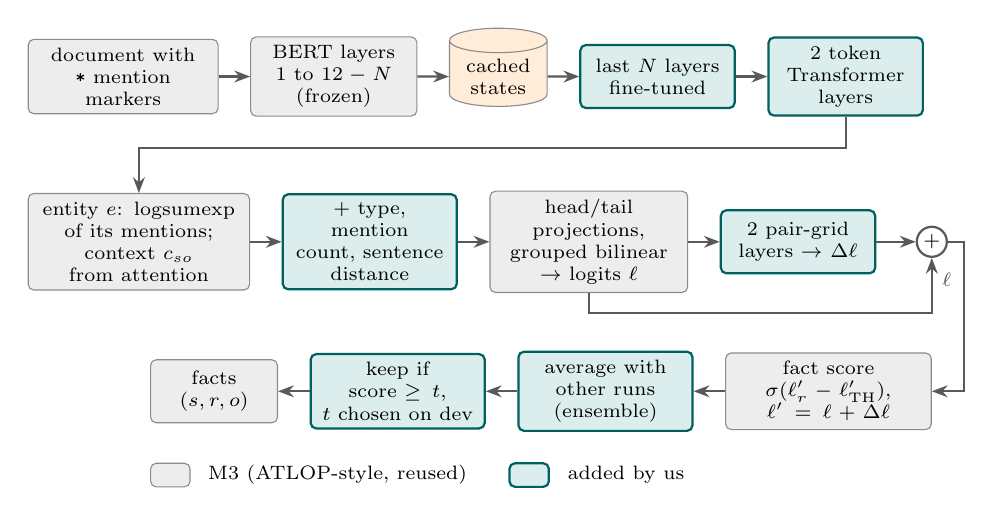
\begin{tikzpicture}[font=\scriptsize, node distance=4mm and 4mm]
\node[reused, text width=2.2cm] (doc) {document with\\ \texttt{*} mention markers};
\node[reused, text width=1.9cm, right=of doc] (low) {BERT layers\\ $1$ to $12-N$\\ (frozen)};
\node[cache, right=of low, minimum height=9mm, text width=1.1cm] (cache) {cached\\ states};
\node[added, text width=1.75cm, right=of cache] (top) {last $N$ layers\\ fine-tuned};
\node[added, text width=1.75cm, right=of top] (tok) {2 token\\ Transformer\\ layers};
\draw[flow] (doc) -- (low); \draw[flow] (low) -- (cache); \draw[flow] (cache) -- (top); \draw[flow] (top) -- (tok);

\node[reused, text width=2.6cm, below=10mm of doc.south west, anchor=north west] (pool) {entity $e$: logsumexp\\ of its mentions;\\ context $c_{so}$ from attention};
\node[added, text width=2.0cm, right=of pool] (feat) {+ type, mention\\ count, sentence\\ distance};
\node[reused, text width=2.3cm, right=of feat] (bil) {head/tail projections,\\ grouped bilinear\\ $\to$ logits $\ell$};
\node[added, text width=1.75cm, right=of bil] (grid) {2 pair-grid\\ layers $\to \Delta\ell$};
\node[circle, draw=black!65, thick, inner sep=1pt, right=5mm of grid] (plus) {$+$};
\draw[flow] (tok.south) -- ++(0,-4mm) -| (pool.north);
\draw[flow] (pool) -- (feat); \draw[flow] (feat) -- (bil); \draw[flow] (bil) -- (grid); \draw[flow] (grid) -- (plus);
\draw[flow] (bil.south) -- ++(0,-2.5mm) -| node[pos=0.8, right] {$\ell$} (plus.south);

\node[reused, text width=2.4cm, below=12mm of plus.south, anchor=north east] (score) {fact score\\ $\sigma(\ell'_r-\ell'_{\mathrm{TH}})$, $\ell'=\ell+\Delta\ell$};
\node[added, text width=2.0cm, left=of score] (ens) {average with\\ other runs\\ (ensemble)};
\node[added, text width=2.0cm, left=of ens] (thr) {keep if score $\ge t$,\\ $t$ chosen on dev};
\node[reused, text width=1.4cm, left=of thr] (facts) {facts\\ $(s, r, o)$};
\draw[flow] (plus.east) -- ++(2mm,0) |- (score.east);
\draw[flow] (score) -- (ens); \draw[flow] (ens) -- (thr); \draw[flow] (thr) -- (facts);

\node[reused, minimum height=3mm, minimum width=5mm, below=5mm of facts.south west, anchor=north west] (k1) {};
\node[right=1mm of k1] (k1t) {M3 (ATLOP-style, reused)};
\node[added, minimum height=3mm, minimum width=5mm, right=4mm of k1t] (k2) {};
\node[right=1mm of k2] {added by us};
\end{tikzpicture}
\caption{The document model. Grey parts are those of M3; the parts in colour are our additions, each switched on or off by a training option so that its gain can be measured. Every part after the encoder is computed for all the entity pairs of a document at once.}\label{fig:docmodel}
\end{figure}

\begin{figure}[htbp]
\centering
\begin{minipage}[t]{0.47\linewidth}
\centering
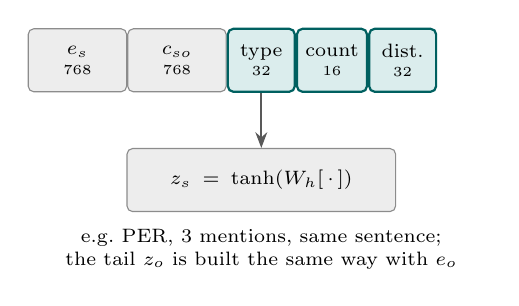
\begin{tikzpicture}[font=\scriptsize, node distance=0mm]
\node[reused, minimum width=1.25cm] (e) {$e_s$\\[-1pt]{\tiny 768}};
\node[reused, minimum width=1.25cm, right=of e] (c) {$c_{so}$\\[-1pt]{\tiny 768}};
\node[added, minimum width=0.85cm, right=of c] (ty) {type\\[-1pt]{\tiny 32}};
\node[added, minimum width=0.85cm, right=of ty] (nm) {count\\[-1pt]{\tiny 16}};
\node[added, minimum width=0.85cm, right=of nm] (di) {dist.\\[-1pt]{\tiny 32}};
\node[reused, below=7mm of ty, text width=3.2cm] (z) {$z_s = \tanh(W_h[\,\cdot\,])$};
\draw[flow] (ty.south) -- (z.north);
\node[below=1mm of z, text width=5.6cm, align=center] {e.g.\ PER, 3 mentions, same sentence;\\ the tail $z_o$ is built the same way with $e_o$};
\end{tikzpicture}\\[1mm]
(a) Pair features
\end{minipage}\hfill
\begin{minipage}[t]{0.47\linewidth}
\centering
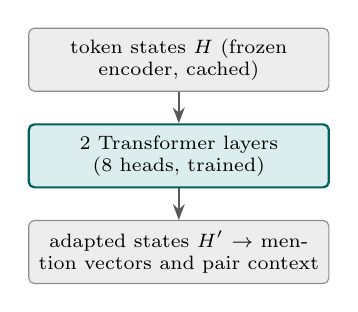
\begin{tikzpicture}[font=\scriptsize, node distance=4mm]
\node[reused, text width=3.6cm] (h) {token states $H$ (frozen encoder, cached)};
\node[added, text width=3.6cm, below=of h] (t) {2 Transformer layers\\ (8 heads, trained)};
\node[reused, text width=3.6cm, below=of t] (o) {adapted states $H'$ $\to$ mention vectors and pair context};
\draw[flow] (h) -- (t); \draw[flow] (t) -- (o);
\end{tikzpicture}\\[1mm]
(b) Token layers
\end{minipage}

\vspace{4mm}
\begin{minipage}{\linewidth}
\centering
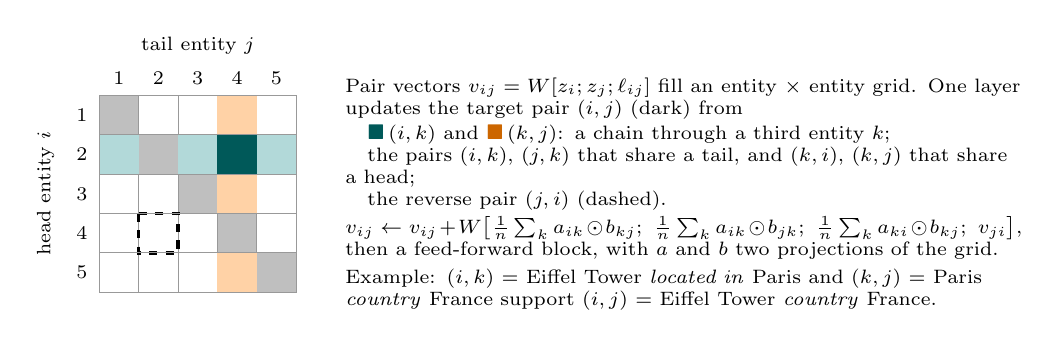
\begin{tikzpicture}[font=\scriptsize]
\def\s{0.5}
\foreach \r in {0,...,4} \foreach \c in {0,...,4} {
  \ifnum\r=\c \fill[black!25] (\c*\s,-\r*\s) rectangle ++(\s,-\s); \fi
  \draw[black!40] (\c*\s,-\r*\s) rectangle ++(\s,-\s);
}
\foreach \c in {0,2,4} \fill[teal!30] (\c*\s,-1*\s) rectangle ++(\s,-\s);
\foreach \r in {0,2,4} \fill[orange!35] (3*\s,-\r*\s) rectangle ++(\s,-\s);
\fill[teal!70!black] (3*\s,-1*\s) rectangle ++(\s,-\s);
\draw[very thick, dashed, black] (1*\s,-3*\s) rectangle ++(\s,-\s);
\foreach \r in {0,...,4} \draw[black!40] (0,-\r*\s) rectangle ++(5*\s,-\s);
\foreach \i in {1,...,5} { \node at (\i*\s-\s/2, 0.22) {\i}; \node at (-0.22, -\i*\s+\s/2) {\i}; }
\node[anchor=south] at (2.5*\s, 0.4) {tail entity $j$};
\node[rotate=90, anchor=south] at (-0.45, -2.5*\s) {head entity $i$};
\node[anchor=west, text width=8.6cm, align=left] at (5*\s+0.5, -1.25) {
  Pair vectors $v_{ij} = W[z_i; z_j; \ell_{ij}]$ fill an entity $\times$ entity grid. One layer updates
  the target pair $(i,j)$ (dark) from\\[1pt]
  \quad\textcolor{teal!70!black}{$\blacksquare$}\,$(i,k)$ and \textcolor{orange!80!black}{$\blacksquare$}\,$(k,j)$: a chain through a third entity $k$;\\
  \quad the pairs $(i,k)$, $(j,k)$ that share a tail, and $(k,i)$, $(k,j)$ that share a head;\\
  \quad the reverse pair $(j,i)$ (dashed).\\[2pt]
  $v_{ij} \leftarrow v_{ij} + W\big[\tfrac1n\textstyle\sum_k a_{ik}\odot b_{kj};\ \tfrac1n\sum_k a_{ik}\odot b_{jk};\ \tfrac1n\sum_k a_{ki}\odot b_{kj};\ v_{ji}\big]$,
  then a feed-forward block, with $a$ and $b$ two projections of the grid.\\[2pt]
  Example: $(i,k)$ = Eiffel Tower \emph{located in} Paris and $(k,j)$ = Paris \emph{country} France
  support $(i,j)$ = Eiffel Tower \emph{country} France.};
\end{tikzpicture}\\[1mm]
(c) Pair-grid reasoning layer (grey diagonal: no pair of an entity with itself)
\end{minipage}

\vspace{4mm}
\begin{minipage}[t]{0.4\linewidth}
\centering
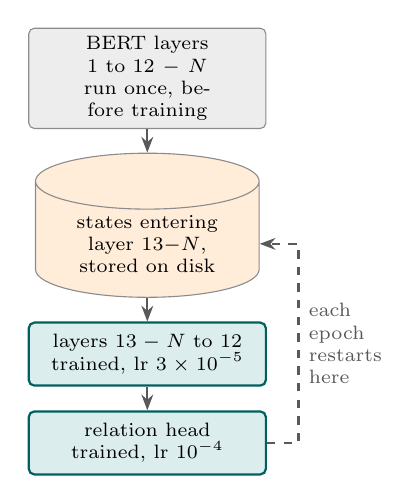
\begin{tikzpicture}[font=\scriptsize, node distance=3mm]
\node[reused, text width=2.8cm] (l1) {BERT layers $1$ to $12-N$\\ run once, before training};
\node[cache, below=of l1, minimum height=10mm, text width=2.7cm] (ca) {states entering\\ layer $13{-}N$,\\ stored on disk};
\node[added, text width=2.8cm, below=of ca] (lt) {layers $13-N$ to $12$\\ trained, lr $3\times10^{-5}$};
\node[added, text width=2.8cm, below=of lt] (hd) {relation head\\ trained, lr $10^{-4}$};
\draw[flow] (l1) -- (ca); \draw[flow] (ca) -- (lt); \draw[flow] (lt) -- (hd);
\draw[flow, dashed] (hd.east) -- ++(4mm,0) |- node[pos=0.25, right, align=left] {each\\ epoch\\ restarts\\ here} (ca.east);
\end{tikzpicture}\\[1mm]
(d) Partial fine-tuning, $N=2$ or $4$
\end{minipage}\hfill
\begin{minipage}[t]{0.55\linewidth}
\centering
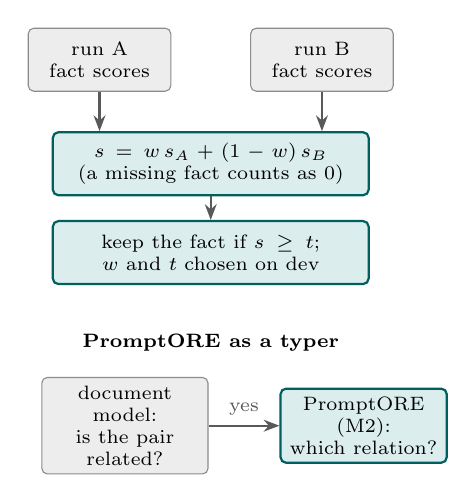
\begin{tikzpicture}[font=\scriptsize, node distance=3mm and 4mm]
\node[reused, text width=1.6cm] (a) {run A\\ fact scores};
\node[reused, text width=1.6cm, right=10mm of a] (b) {run B\\ fact scores};
\node[added, text width=3.8cm, below=5mm of $(a.south)!0.5!(b.south)$, anchor=north] (m) {$s = w\,s_A + (1-w)\,s_B$\\ (a missing fact counts as 0)};
\draw[flow] (a.south) -- (a.south |- m.north); \draw[flow] (b.south) -- (b.south |- m.north);
\node[added, text width=3.8cm, below=of m] (t) {keep the fact if $s \ge t$;\\ $w$ and $t$ chosen on dev};
\draw[flow] (m) -- (t);
\node[below=5mm of t, font=\scriptsize\bfseries] (lab) {PromptORE as a typer};
\node[reused, text width=1.9cm, below=2mm of lab.south west, anchor=north west, xshift=-4mm] (d) {document model:\\ is the pair related?};
\node[added, text width=1.9cm, right=9mm of d] (p) {PromptORE (M2):\\ which relation?};
\draw[flow] (d) -- node[above] {yes} (p);
\end{tikzpicture}\\[1mm]
(e) Ensembles and PromptORE as a typer
\end{minipage}
\caption{The additions of the document model in detail. Grey: M3 parts; teal: trained parts we added; orange cylinder: cached states.}\label{fig:docparts}
\end{figure}


\subsubsection{M4: LLM representations of a pair in PromptORE}\label{sec:llm}
M4 is described last because it was added at the end of the project and extends M1 and M2, not the document model; it scores between M2 and M3. A large language model is not run end to end: it replaces or completes the \emph{representation of a pair} inside M1 and M2, and everything else (candidates, context, train sample, detector, classifiers, clusters, thresholds) is the code of M1 and M2, so the gap with PromptORE measures the representation only. The LLM reads the same context as PromptORE and the two entity names, and answers one line, \texttt{relation | head type | tail type}, where the relation is a free phrase of one to five words or \texttt{none}; it never sees the 96 relations or a label. The answer is embedded with a sentence encoder (\texttt{all-mpnet-base-v2}~\cite{reimers2019sbert}). We compared the hidden state and the answer of a local \texttt{Qwen2.5-3B-Instruct}~\cite{qwen2024qwen25}, the answer of DeepSeek (\texttt{deepseek-chat}~\cite{deepseek2024v3}) through its API, and the concatenation of the BERT \texttt{[MASK]} state (centred, L2-normalised) with that answer. To bound the API cost, the method is trained on 1,000 train documents (89,484 sampled pairs), and the dev pairs whose BERT detection probability is below 0.02 are not sent to the API and get no fact (92,981 of the 187,939 dev pairs; the threshold costs 0.1 F1 point on the 100 dev documents used to choose it, which were all sent).

\subsubsection{Corpus graph}\label{sec:graph}

Entities linked to the same Wikidata item become one node across documents; dates and numbers merge on their normalized text; other entities stay local to their document, since merging them on the name could join different entities. Facts with the same (head node, relation, tail node) become one edge whose confidence is the noisy-or of its document scores, $1-\prod_d (1-s_d)$, so that a fact found in several documents becomes more certain. Each edge keeps its supporting documents and scores. We found and fixed a bug where placeholder identifiers of the dataset (\texttt{\#ignored\#} for dates) were taken for Wikidata items and merged all dates into one node. We also built an HTML viewer that draws the gold graph next to the predicted graph of a run, by document or around one entity, with correct, missed and wrong edges and the evidence sentences of each fact.

\subsection{Evaluation methods}\label{sec:evaluation}

With other team members working on other methods, we wrote a shared benchmark and evaluator: every method writes prediction files in one format, one script computes every metric and adds a row to a common leaderboard. The metrics are:

\begin{itemize}
\item \textbf{Micro precision, recall and F1} over facts, and \textbf{Ign F1}, the F1 without the facts already present in train, which guards against memorization (the two key metrics, as in DocRED papers);
\item \textbf{Detection F1} (does the pair have at least one relation?) and \textbf{typing F1} (on the gold related pairs that a method detects, does it choose the right relations?), to answer Q2;
\item \textbf{Macro F1} by relation frequency (10 frequent relations, medium, rare with fewer than 200 train facts), and F1 on pairs inside one sentence and across sentences;
\item \textbf{Graph metrics:} precision, recall and F1 over distinct triples after merging documents, precision at the $N$ most confident edges, and precision by number of supporting documents;
\item \textbf{Reliability:} mean and standard deviation over seeds, a 95\% bootstrap interval over documents, and a paired bootstrap test between two runs.
\end{itemize}

\textbf{Protocol.} Test was scored during development for some runs, which a final result should not allow. Since then, runs are scored on dev only, and the test scores reported below are marked \emph{provisional} until one final test run. Dev and test agree within 0.3 point for every document model, so the dev choices did not overfit.

\subsection{Experiments and results}\label{sec:results}

\subsubsection{Comparison of the methods (Q1)}

Table~\ref{tab:main} gives the test scores. The supervised document models beat PromptORE by a wide margin: the final ensemble reaches 75.0 F1, against 50.4 for M2 and 45.9 for M1. The gaps are significant: by paired bootstrap on dev, M3 beats M2 by 9.2 points (95\% interval 7.8 to 10.4) and M2 beats M1 by 4.6 points (4.1 to 5.2), far above the seed standard deviation (0.1 to 0.5 point). Our best model, BERT-base partly fine-tuned on a laptop, is 2.6 points below the published fully fine-tuned RoBERTa-large ATLOP (77.6). Without reading the text, the structure of the document is worth little: M0' gains 3.0 test F1 over M0 (dev: +4.3, paired bootstrap interval +3.5 to +5.1), and stays 24 points below PromptORE, so almost all of the F1 of the other methods comes from the text.

\begin{table}[htbp]
\caption{Test scores of each method (provisional, see Section~\ref{sec:evaluation}). Mean $\pm$ standard deviation over 3 seeds when available.}\label{tab:main}
\centering
\begin{tabular}{@{}lccccc@{}}
\toprule
Method & F1 & Ign F1 & Detect. F1 & Typing F1 & Graph F1 \\
\midrule
M0 type-pair baseline & 18.86 & 17.80 & 28.14 & 61.98 & 19.42 \\
M0' structural baseline & 21.90 $\pm$ 0.06 & 20.39 & 34.22 & 60.20 & 22.40 \\
M1 PromptORE + clusters & 45.93 $\pm$ 0.38 & 43.56 & 51.29 & 83.19 & 46.01 \\
M2 PromptORE + classifier & 50.41 $\pm$ 0.14 & 48.07 & 53.21 & 88.91 & 50.70 \\
M3 ATLOP-style, frozen & 57.70 $\pm$ 0.10 & 56.76 & 60.14 & 92.17 & 59.20 \\
Doc. model, frozen & 66.04 $\pm$ 0.14 & 64.53 & 68.45 & 93.15 & 66.88 \\
Doc. model, 4 layers tuned & 73.55 & 72.27 & 75.49 & 94.80 & 74.34 \\
Final ensemble & \textbf{74.99} & \textbf{73.83} & \textbf{76.51} & \textbf{95.46} & \textbf{75.84} \\
\botrule
\end{tabular}
\end{table}

PromptORE is still useful in two ways. As a typer on the pairs detected by the document model, M2 rises from 49.2 to 60.9 dev F1 and M1 from 44.6 to 55.7: about 11 points of PromptORE were lost at detection alone. As a member of an ensemble, M2 adds +0.5 dev F1 because it finds facts that the supervised models miss: in v1, M3 and M2 share 5,967 correct facts but each finds about 2,500 that the other misses.

\subsubsection{What each change brings}

Fig.~\ref{fig:progression} and Table~\ref{tab:gains} trace the dev F1 after each change, and the changes we dropped.

\begin{figure}[htbp]
\centering
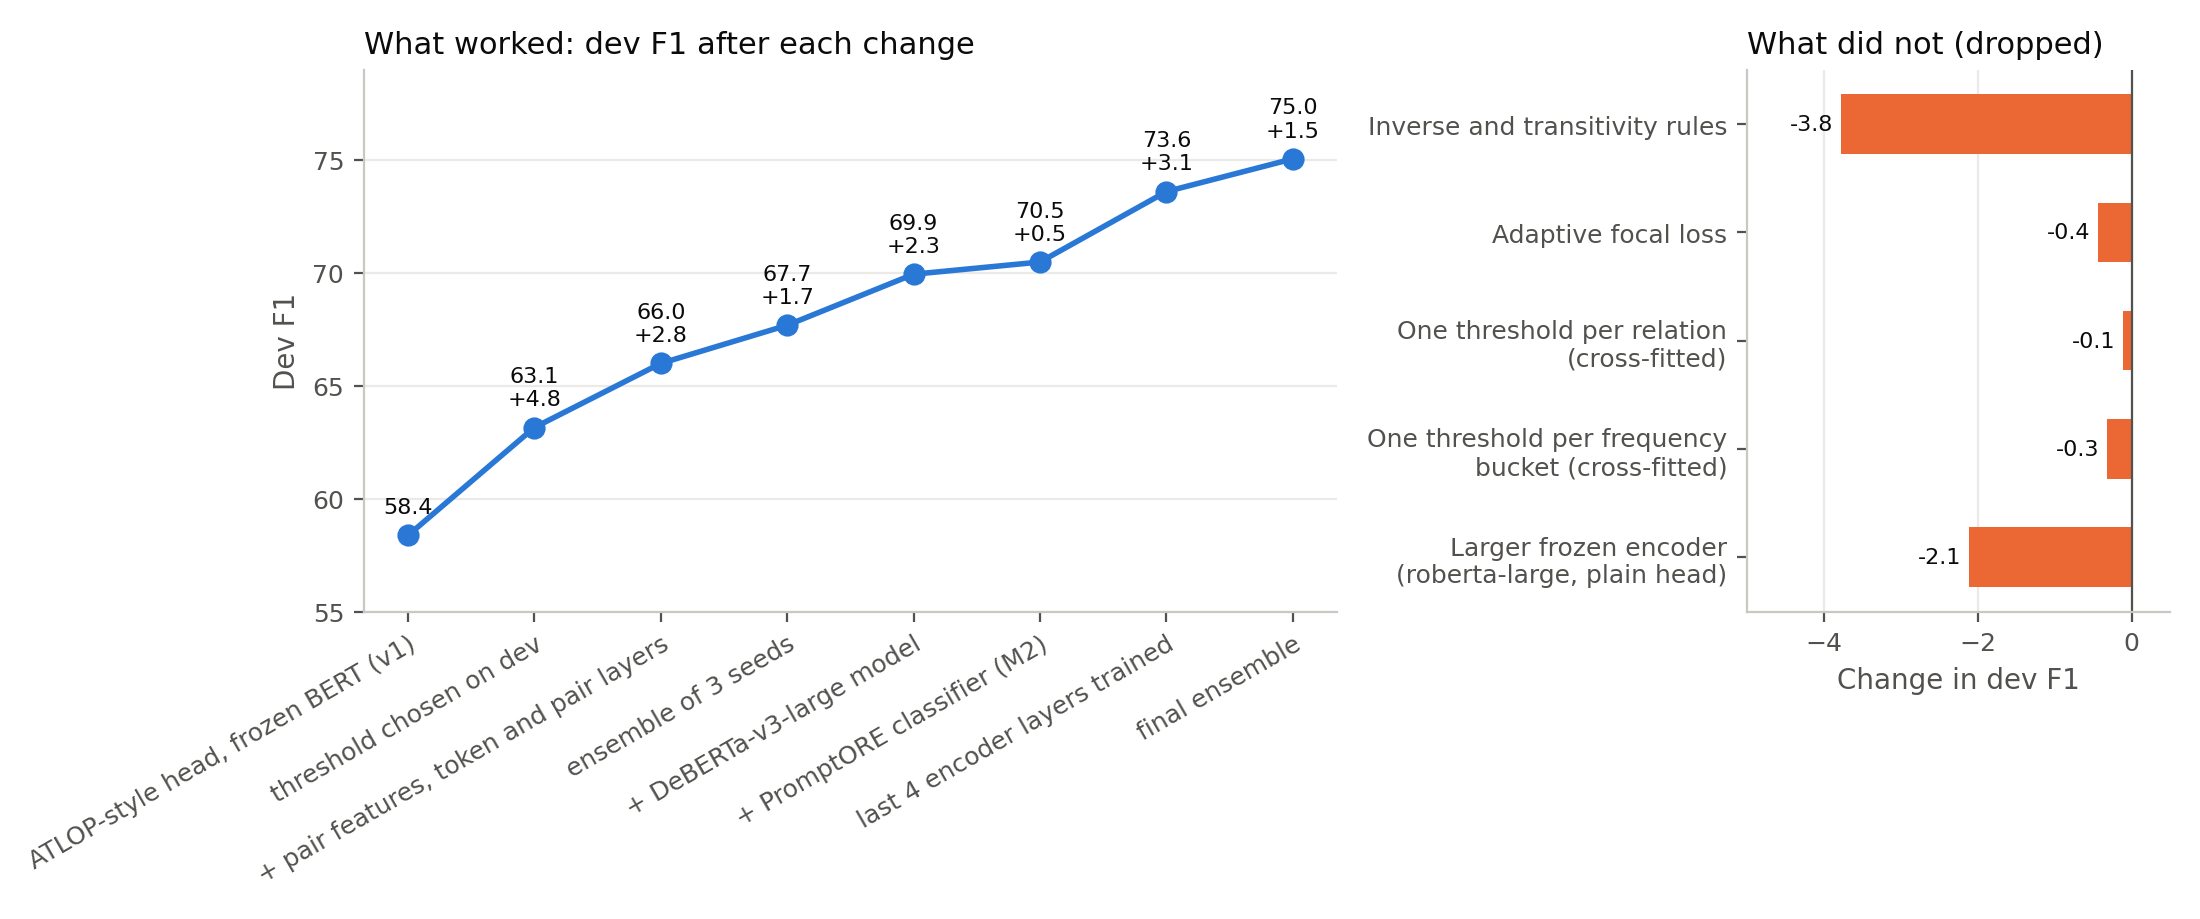
\includegraphics[width=\linewidth]{figures/progression_dev_f1.png}
\caption{Left: dev F1 after each change, from M3 to the final ensemble. Right: changes that did not help and were dropped.}\label{fig:progression}
\end{figure}

\begin{table}[htbp]
\caption{Gain of each change on dev F1 (one run, seed 0, unless stated otherwise).}\label{tab:gains}
\centering
\begin{tabular}{@{}lrr@{}}
\toprule
Change & Dev F1 & Gain \\
\midrule
M3, ATLOP-style head on frozen BERT (3 seeds) & 58.37 & \\
Fact threshold chosen on dev (cross-fitted: 63.04) & 63.15 & +4.78 \\
+ pair features, 2 token layers, 2 pair layers & 65.99 & +2.84 \\
Ensemble of 3 seeds & 67.68 & +1.69 \\
+ DeBERTa-v3-large document model & 69.94 & +2.26 \\
+ PromptORE classifier (M2) & 70.48 & +0.54 \\
Last 4 encoder layers trained (one model) & 73.60 & +3.12 \\
Final ensemble (tuned models and frozen ensemble) & 75.05 & +1.45 \\
\midrule
\multicolumn{3}{@{}l}{\emph{Dropped}} \\
Inverse and transitivity rules (on M3) & 54.98 & $-3.77$ \\
roberta-large, frozen, plain head (against bert-base) & 61.04 & $-2.11$ \\
Adaptive focal loss instead of the adaptive threshold loss & 62.72 & $-0.43$ \\
One threshold per relation (cross-fitted) & 62.93 & $-0.11$ \\
\midrule
\multicolumn{3}{@{}l}{\emph{Post-processing of the final ensemble (cross-fitted on dev)}} \\
Rules from train: entity types, functional relations & 75.11 & +0.05 \\
One threshold per relation frequency bucket & 74.74 & $-0.32$ \\
Rescorer on train rules and document features & 75.36 & +0.31 \\
\botrule
\end{tabular}
\end{table}

\begin{itemize}
\item \textbf{The threshold is the largest cheap gain.} M3 was too cautious (precision 72.9, recall 49.2): its learned threshold was right for its training loss, not for F1. A threshold chosen on dev trades precision for recall, and the gain holds when cross-fitted. One threshold per relation overfits dev (+1.4 on the folds it was tuned on, $-0.1$ cross-fitted).
\item \textbf{The three architectural additions add up only partly:} +2.84 together, against +3.48 for the sum of their separate gains (pair features +1.04, token layers +1.60, pair layers +0.84). Combining token layers with another part diverged at learning rate $3\times10^{-4}$; $10^{-4}$ is stable.
\item \textbf{A larger frozen encoder does not help by itself} (roberta-large 61.0, DeBERTa-v3-large 63.3 against 63.2 for BERT-base under the plain head). DeBERTa only helps under the full model (+1.0) and mostly as an ensemble member: a second encoder brings more (+2.6 on test) than two more seeds of the same encoder (+1.4).
\item \textbf{Partial fine-tuning is the largest single gain:} training the last 2 layers gives 71.0 dev F1, the last 4 layers 73.6, against 66.0 for the frozen model. Macro F1 on test rises from 48.5 to 59.4: rare relations gain the most.
\item \textbf{Inference rules hurt.} Adding inverse facts (``part of'' implies ``has part'') and the country implied by ``located in'' lowers F1 by about 4 points for every method: Re-DocRED does not annotate every inferred fact, so the rules add as many false facts as true ones.
\item \textbf{The adaptive focal loss} of KD-DocRE~\cite{tan2022kddocre}, meant for the long tail, did not improve micro or macro F1 in our frozen setting.
\item \textbf{Post-processing the final ensemble brings nothing established.} We rescored its facts down to a score of 0.05 (the candidates hold 88\% of the gold facts, against 72\% kept): hard rules mined from train (relation and entity types never seen together, one tail for functional relations), one threshold per frequency bucket, and a gradient boosting rescorer fitted on four folds of dev and applied to the fifth, whose features are the member scores, the other relations of the pair and of the head, the reverse fact, the type statistics, two-step chain rules mined from train (386 rules), the sentence distance and the predictions of the other documents for the same Wikidata fact. The best variant gains +0.31 dev F1, but a paired bootstrap interval includes 0 and a second fold draw gives +0.07. Only a feature telling whether the Wikidata fact is in the train graph gives a significant gain (+0.4 to +0.5), and it is mostly memorisation (+0.25 Ign F1). The pair-grid layers, the type inputs and the encoder already carry this information; the remaining errors are pairs with low scores everywhere, which no score feature can recover.
\end{itemize}

\subsubsection{An LLM inside PromptORE (M4)}

M4 has no test run and was trained on 1,000 train documents, so it is compared on dev with PromptORE recomputed on the same 1,000 documents (Table~\ref{tab:llm}; one seed). Adding the DeepSeek answer to the BERT state gains 9.2 F1 with the classifier (paired bootstrap interval +8.0 to +10.3) and 8.7 with clusters (+7.7 to +9.7). With a third of the train documents, both rows are above PromptORE trained on all 3,053 (49.2 and 44.6), but below M3 (58.4). The gain is mostly on detection (50.6 to 59.2) and on rare relations (macro F1 26.3 to 39.1), and on pairs that share no sentence (43.2 to 53.1 F1). On the smaller train\_debug/dev\_debug split (300 and 100 documents), the answer alone is no better than BERT (+0.65, interval $-2.5$ to $+4.1$), so the gain comes from combining two representations that carry different information. The local 3B model is worse than BERT, as a hidden state (37.0 against 43.0 with the classifier) and as an answer (28.8). Two uses of the LLM fail: naming the BERT clusters with one of the 96 relations from eight of their pairs gives 22.8 F1 against 37.6 with the train labels, and using no label at all (a pair is related when the answer is not \texttt{none}) gives 17.0 F1, the level of M0, because DeepSeek answers \texttt{none} for 49\% of the related pairs.

\begin{table}[htbp]
\caption{M4 against PromptORE, both trained on the same 1,000 train documents, dev scores, seed 0.}\label{tab:llm}
\centering
\begin{tabular}{@{}lccccc@{}}
\toprule
Representation, typing & F1 & Ign F1 & Detect. F1 & Typing F1 & Macro F1 \\
\midrule
BERT (PromptORE), clusters (M1) & 43.16 & 41.17 & 49.16 & 81.50 & 18.67 \\
BERT (PromptORE), classifier (M2) & 46.82 & 44.65 & 50.62 & 86.19 & 26.31 \\
BERT + DeepSeek answer, clusters & 51.86 & 49.88 & 57.81 & 84.71 & 29.21 \\
BERT + DeepSeek answer, classifier & \textbf{55.98} & \textbf{54.03} & \textbf{59.18} & \textbf{90.11} & \textbf{39.06} \\
\botrule
\end{tabular}
\end{table}

\subsubsection{Detection against typing (Q2)}

Fig.~\ref{fig:detection} confirms the hypothesis of the project. Once a pair is known to be related, every method that reads the text picks the right relation most of the time (typing F1 83 to 95), but deciding which of the about 390 pairs of a document are related is much harder (detection F1 51 to 77). On dev, 89\% of the facts missed by M3 and M2 belong to pairs that are never predicted, and 80\% to 86\% of their false facts are on pairs without any gold relation. From M3 to the final ensemble, detection F1 gained 16 points and typing F1 only 3, and the LLM answer of M4 also helps PromptORE mostly at detection (+8.6 against +3.9 for typing). The same gap holds for the baselines that read no text (M0': detection 34.2, typing 60.2): the entity types alone say which relation a related pair has much better than whether it has one.

\begin{figure}[htbp]
\centering
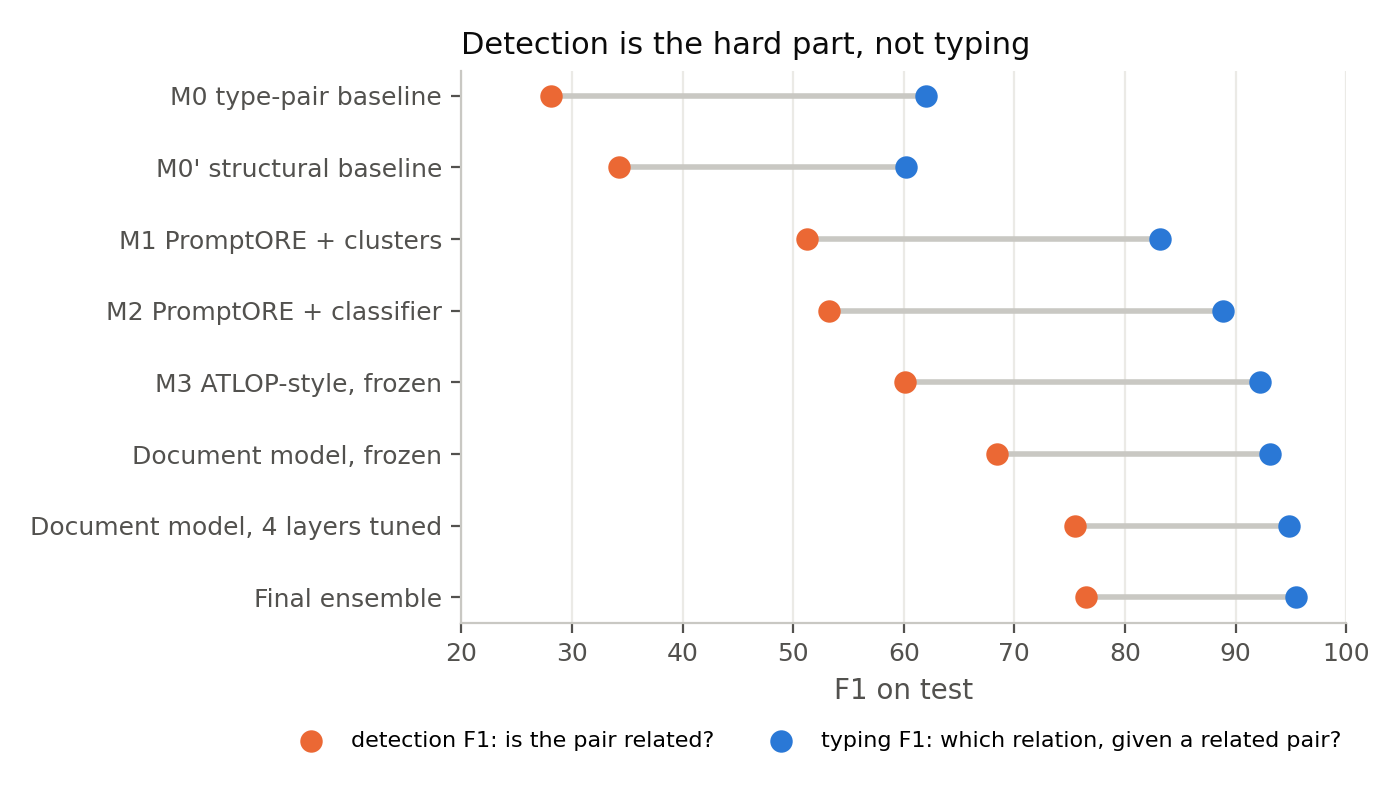
\includegraphics[width=0.85\linewidth]{figures/detection_vs_typing.png}
\caption{Detection F1 and typing F1 on test for each method.}\label{fig:detection}
\end{figure}

The error analyses on dev give the linguistic side of these failures:
\begin{itemize}
\item \textbf{Distance:} M2 precision falls from 57.7 on pairs in the same sentence to 39.0 on pairs three or more sentences apart, since its prompt only sees the sentences of the mentions; M3 reads the whole document and keeps a precision of 70 to 75 at every distance.
\item \textbf{Inferred relations:} the most missed relations are P131 (located in), P17 (country), P150 (contains), P527 (has part) and P361 (part of), geographic and part-of hierarchies that annotators often infer rather than read in the text. P131 and P17 also give a third of the false positives of the ensemble.
\item \textbf{Entity types and length:} M3 recall is 61 on LOC--LOC pairs but 31 on PER--PER pairs, and 55 in documents with fewer than 15 entities against 44 with 25 or more.
\item \textbf{Annotation gaps} explain few errors: only 50 of the 3,158 false facts of M3 are the inverse of a gold fact, and 113 are gold in another document.
\end{itemize}

\begin{figure}[htbp]
\centering
\includegraphics[width=0.85\linewidth]{figures/relation_frequency.png}
\caption{Macro F1 on test by relation frequency.}\label{fig:frequency}
\end{figure}

Rare relations remain the weakest point (Fig.~\ref{fig:frequency}): macro F1 on relations with fewer than 200 train facts is 8 for M1, 21 for M2, 20 for M3 and 47 for the final ensemble. M1 suffers most because a cluster is named after the majority of its train pairs, and a rare relation rarely dominates a cluster.

\subsubsection{Labels needed (Q3)}

We trained M1, M2 and the frozen document model on a random share of the train documents, drawn twice per share with the same documents for every method, and scored them on dev (Table~\ref{tab:labels}, Fig.~\ref{fig:labels}).

\begin{table}[htbp]
\caption{Dev F1 with a share of the 3,053 train documents (mean of 2 draws; the draws differ by less than 0.7 point). The 100\% document model is the mean of 3 seeds.}\label{tab:labels}
\centering
\begin{tabular}{@{}lrrr@{}}
\toprule
Train documents & M1 & M2 & Document model, frozen \\
\midrule
5\% (153) & 34.15 & 39.94 & 52.10 \\
10\% (305) & 38.91 & 42.87 & 56.26 \\
25\% (763) & 42.22 & 45.88 & 60.73 \\
50\% (1,526) & 43.99 & 47.87 & 64.23 \\
100\% (3,053) & 44.15 & 49.24 & 66.18 \\
\botrule
\end{tabular}
\end{table}

\begin{figure}[htbp]
\centering
\includegraphics[width=0.8\linewidth]{figures/label_efficiency_dev.png}
\caption{Dev F1 against the share of labeled train documents (log scale).}\label{fig:labels}
\end{figure}

Trained on 153 documents, the supervised document model already beats both PromptORE methods trained on all 3,053 (52.1 against 49.2 and 44.2). With 5\% of the documents, M1, M2 and the document model keep 77\%, 81\% and 79\% of their full F1. M1 saturates first (+0.2 from 50\% to 100\%) because its clusters do not use the labels, which only name the clusters and train the detector. PromptORE does not win in the low-label regime as its design suggests, because on this data the labels mostly serve detection, and a prompt over the mention sentences is a weaker detection signal than a model that reads the whole document.

\subsubsection{Graph quality and calibration (Q4)}

The graph of the final ensemble on test has 5,179 nodes and 13,792 edges, with a graph F1 of 75.8. Repetition across documents is a strong signal (Fig.~\ref{fig:support}): an edge stated by one document is correct 79.2\% of the time, by two documents 97.7\%, by three or more 99.1\%. Edges supported by several documents are few, however, so most of the graph rests on single documents.

\begin{figure}[htbp]
\centering
\includegraphics[width=0.8\linewidth]{figures/graph_precision_by_support.png}
\caption{Edge precision on test by number of documents that state the edge.}\label{fig:support}
\end{figure}

To know whether the scores can be trusted, we grouped the dev facts of each run into ten score bins and compared the share of correct facts with the mean score of each bin (Fig.~\ref{fig:calibration}). For every run, precision rises steadily with the score, so the scores rank facts and edges well. They are not calibrated probabilities, though: the final ensemble is under-confident (facts with a mean score of 0.25 are correct 40\% of the time, and facts scored above 0.9 are correct 99\% of the time), the partly fine-tuned model is over-confident at the top (facts with a mean score of 0.85 are correct 76\% of the time), and M2 lies close to the diagonal. A calibration step fitted on dev, such as isotonic regression, would fix the values without changing the ranking.

\begin{figure}[htbp]
\centering
\includegraphics[width=0.6\linewidth]{figures/calibration_dev.png}
\caption{Reliability diagram on dev: share of correct facts against the mean fact score of each score bin.}\label{fig:calibration}
\end{figure}

\subsubsection{Difficulties and how we handled them}

Table~\ref{tab:difficulties} summarizes the main obstacles of the project and how each one was handled.

\begin{table}[htbp]
\caption{Main difficulties of the project and how we handled them.}\label{tab:difficulties}
\centering
\small
\begin{tabular}{@{}p{0.3\linewidth}p{0.36\linewidth}p{0.26\linewidth}@{}}
\toprule
Difficulty & What we did & Outcome \\
\midrule
PromptORE assumes one relation per instance; 94\% of our pairs have none & Reproduced the paper first, then added a detector & Detection becomes the measured bottleneck \\
Two datasets made comparisons inconsistent & Kept Linked-Re-DocRED only & Same documents for every method \\
1.19 million train pairs, one BERT pass per pair for PromptORE & Sample of 3 unrelated pairs per related pair, with weights; embeddings cached & 271,232 embeddings computed once \\
No server GPU & Cached encoder states; training of the last 4 layers from cached lower states & +7.5 test F1 for one model \\
Several people, several methods & Shared benchmark, evaluator and leaderboard & One script for every number \\
The first document model was too cautious (precision 73, recall 48) & Fact threshold chosen on dev, checked by cross-fitting & +4.8 dev F1 \\
Test used during development & Dev only until one final test run & Test scores marked provisional \\
Training diverged & Learning rate $3\times10^{-4}$ lowered to $10^{-4}$ & Stable training \\
\botrule
\end{tabular}
\end{table}

%% ---------------------------------------------------------------------------
\section{Conclusion}\label{sec:conclusion}

We compared unsupervised and supervised relation extraction on documents whose entities are known, with one benchmark and one evaluator, and assembled the predicted facts into a knowledge graph. The answers to our questions are clear. \textbf{Q1:} PromptORE stays 25 points below the best supervised model, but is useful as a typer and as an ensemble member; completing its representation with the answer of an LLM gains 9 dev F1 points. \textbf{Q2:} detection, not typing, is the bottleneck for every method. \textbf{Q3:} the supervised document model needs few labels: 5\% of the train documents are enough to beat PromptORE trained on all of them. \textbf{Q4:} the graph reaches 75.8 F1, edges confirmed by several documents are almost always right, and scores rank facts reliably but need calibration to be read as probabilities. On a laptop, partial fine-tuning and ensembles bring a BERT-base model to 75.0 F1, 2.6 points below the published fully fine-tuned RoBERTa-large ATLOP.

\subsection{Contribution of each member}

All three members wrote this report and prepared the presentation.

\paragraph{Xingran Quan.} Designed the global evaluation methodology: the shared benchmark and evaluator on which every method of this report is scored, with fixed subsets, one prediction format, one script and Colab cell for every metric, and a common leaderboard. Implemented the type-pair baseline (M0), reproduced PromptORE on FewRel NYT and PubMed and compared LLM states and phrases with it, and designed and ran the LLM representations of a pair inside PromptORE (M4), with a local model and the DeepSeek API.
The hardest part was to make several people, scripts and datasets comparable; the most interesting, that an LLM answer helps PromptORE mostly through detection.

\paragraph{Laurent Zhu.} Adapted PromptORE to documents (M1 and M2: context sentences, detector, cluster naming and supervised classifier). Implemented the ATLOP-style classifier (M3) and everything added to it to reach the best F1: the document-level model, the threshold chosen on dev, the pair features, the token and pair-grid layers, the other encoders, the partial fine-tuning of the last encoder layers from cached states, the ensembles and PromptORE as a typer. Also built the corpus graph and its HTML viewer, extended the shared evaluator (Ign F1, detection and typing F1, graph metrics, seeds, bootstrap intervals and paired tests), ran the error analyses (by distance, entity types and relation frequency) and the experiments on labels (Q3) and calibration (Q4).
The hardest part was to train a document model without a GPU, which led to caching the lower encoder layers; the most interesting, that each gain came from reading the errors of the previous model, and that several logical ideas, such as inference rules, lowered the score.

\paragraph{Yuchen Yang.} Implemented the structural baseline (M0'): a detector and one classifier per relation, with exactly the shape of M2, on structural features only (entity types, sentence distance, number of mentions, Wikidata links), so that the gap to M2 measures what reading the text is worth. It gains 4.3 dev F1 over M0 and first showed the pattern of every method, weak detection (34 F1) and strong typing (60 F1); per-relation thresholds overfit (12.4 against 23.5 F1).
The hardest part was to get a useful signal without reading any text; the most interesting, that the structure alone already shows where the difficulty of the task lies.

\subsection{Limits}

The entities are given: a real system must also find, resolve and link them, and its errors would add to ours. We use one dataset, in English, built from Wikipedia introductions. Most single-model results come from one seed; seeds of the same model differ by about 0.3 point on dev, so gains below 0.5 point are not established. Encoders were never fully fine-tuned, and partial fine-tuning was only tried on BERT-base with 2 and 4 layers. M4 was trained on 1,000 train documents with one seed, depends on an external model that may change, and has no test score. The ensemble weights and thresholds are chosen on dev, which makes the dev scores slightly optimistic. Re-DocRED still misses some true facts, so precision may be slightly underestimated, although our checks suggest the effect is small.

\subsection{Perspectives}

Full fine-tuning of a large encoder on a GPU, as in ATLOP and DREEAM, should close most of the remaining gap; DREEAM would also give evidence sentences for each fact, useful to justify the edges of the graph. Rare relations could benefit from class-balanced losses, and M1 from soft cluster naming with several relations per cluster. The edge scores should be calibrated on dev. M4 shows that an LLM answer completes the PromptORE representation; it should be trained on all train documents with several seeds, scored on test, and tried as an input of the document model, while naming clusters with an LLM did not work. Finally, replacing the gold entities by predicted ones would measure the cost of the full pipeline.

\bibliography{references}

\end{document}
